\chapter{Path Planning}\label{chap:pathplanning}
Path-planning is an important primitive for autonomous mobile robots that lets robots find the shortest---or otherwise optimal---path between two points. Optimal paths could be paths that minimize the amount of turning, the amount of braking or whatever a specific application requires. Algorithms to find a shortest path are important not only in robotics, but also in network routing, video games and understanding protein folding.

Path-planning requires a map of the environment and the robot to be aware of its location with respect to the map. We will assume for now that the robot is able to localize itself,  is equipped with a map, and capable of avoiding temporary obstacles on its way. How to create a map, how to localize a robot, and how to deal with uncertain position information will be major foci of the reminder of this  book. The goals of this chapter are to

\begin{itemize}
\item introduce suitable map representations,
\item explain basic path-planning algorithms  ranging from Dijkstra, to A*, D* and RRT,
\item introduce variations of the path-planning problem, such as coverage path planning.
\end{itemize}

\section{Map representations}\label{sec:maps}
In order to plan a path, we somehow need to represent the environment in the computer. We differentiate between two complementary approaches: discrete and continuous approximations. In a discrete approximation, a map is sub-divided into chunks of equal (e.g., a grid or hexagonal map) or differing sizes (e.g., rooms in a building). The latter maps are also known as \emph{topological maps}.\index{Topological map} Discrete maps lend themselves well to a graph representation. Here, every chunk of the map corresponds to a vertex (also known as ``node''), which are connected by edges, if a robot can navigate from one vertex to the other. For example a road-map is a topological map, with intersections as vertices and roads as edges, labeled with their length (Figure \ref{fig:pathproblem}). Computationally, a graph might be stored as an adjacency or incidence list/matrix. A continuous approximation requires the definition of inner (obstacles) and outer boundaries, typically in the form of a polygon, whereas paths can be encoded as sequences of points defined by real numbers. Despite the memory advantages of a continuous representation, discrete maps are the dominant representation in robotics.

For mapping obstacles, the most common map is the \emph{occupancy grid} map\index{Occupancy grid}. In a grid map, the environment is discretized into squares of arbitrary resolution, e.g. 1cm x 1cm, on which obstacles are marked. In a probabilistic occupancy grid, grid cells can also be marked with the probability that they contain an obstacle. This is particularly important when the position of the robot that senses an obstacle is uncertain. Disadvantages of grid maps are their large memory requirements as well as computational time to traverse data structures with large numbers of vertices. A solution to this is storing the grid map as \emph{k-d tree}.\index{k-d tree (data structure)} A k-d tree recursively breaks the environment into $k$ pieces. For $k=4$, an area is broken into four pieces. Each of these pieces is again broken into four pieces and so on, until the desired resolution is reached. These pieces can easily be stored in a graph with each vertex having four children, which are the four pieces the vertex is broken into, or is a leaf of the tree. What makes this data structure attractive is that not all vertices need to be broken down to the smallest possible resolution. Instead only areas, which contain obstacles need to be further broken down. A grid map containing obstacles and the corresponding k-d tree, here a quadtree, are shown in Figure \ref{fig:gridvskdtree}. There is no silver bullet, and each application might require a different solution that could be a combination of different map types.

\begin{figure}
\centering
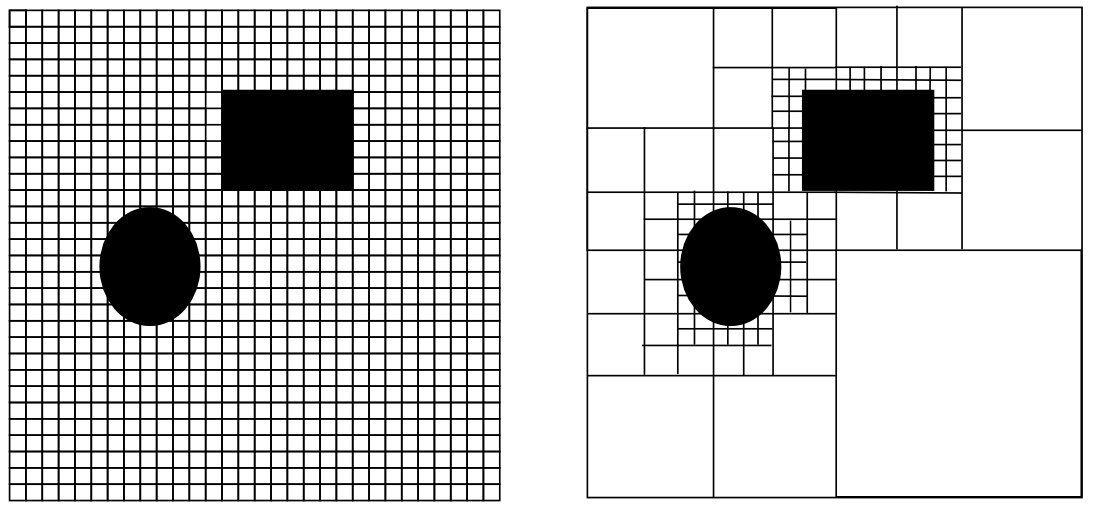
\includegraphics[width=\textwidth]{figs/gridvskdtree.png}
\caption{A grid map and its corresponding quadtree (k-d tree).\label{fig:gridvskdtree}}
\end{figure}


There exist also every possible combination of discrete and continuous representation. For example, roadmaps for GPS systems are stored as topological maps that store the GPS coordinates of every vertex, but might also contain overlays of aerial and street photography or even 3D point clouds stored in a 8-d tree, also known as a \emph{Octree}\index{Octree}. These different maps are then used at different stages of the path planning stage. 


\section{Path-Planning Algorithms}
The problem to find a ``shortest'' path from one vertex to another through a connected graph is of interest in multiple domains, most prominently in the internet, where it is used to find an optimal route for a data packet. The term ``shortest'' refers here to the minimum cumulative edge cost, which could be physical distance (in a robotic application), delay (in a networking application) or any other metric that is important for a specific application. An example graph with arbitrary edge-lengths is shown in Figure \ref{fig:pathproblem}. 

\begin{figure}[!htb]
\centering
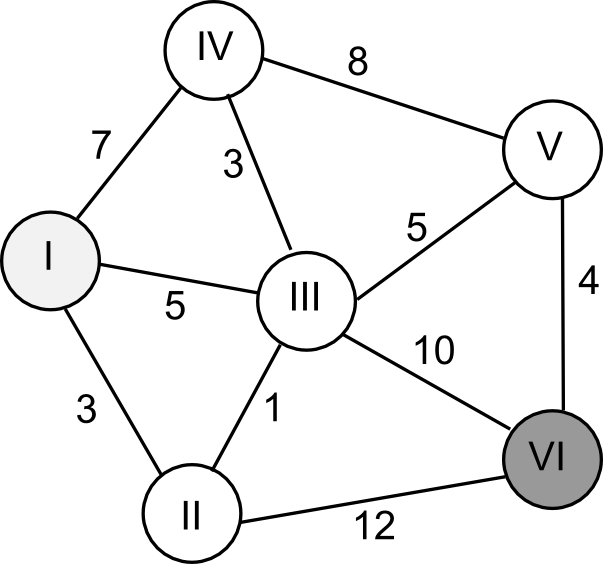
\includegraphics[width=0.6\textwidth]{figs/dijkstra}
\caption{A generic path planning problem from vertex I to vertex VI. The shortest path is I-II-III-V-VI with length 13. \label{fig:pathproblem}}
\end{figure}

\subsection{Robot embodiment}
In order to deal with the physical embodiment of the robot, which complicates the path-planning process, the robot is reduced to a point-mass and all the obstacles in the environment are grown by half of the longest extension of the robot from its center. This representation is known as configuration space \index{Configuration space}as it reduces the representation of the robot to its $x$ and $y$ coordinates in the plane. An example is shown in Figure \ref{fig:cspace}. The configuration space can now either be used as a basis for a grid map or a continuous representation. 

\begin{figure}[!htb]
\centering
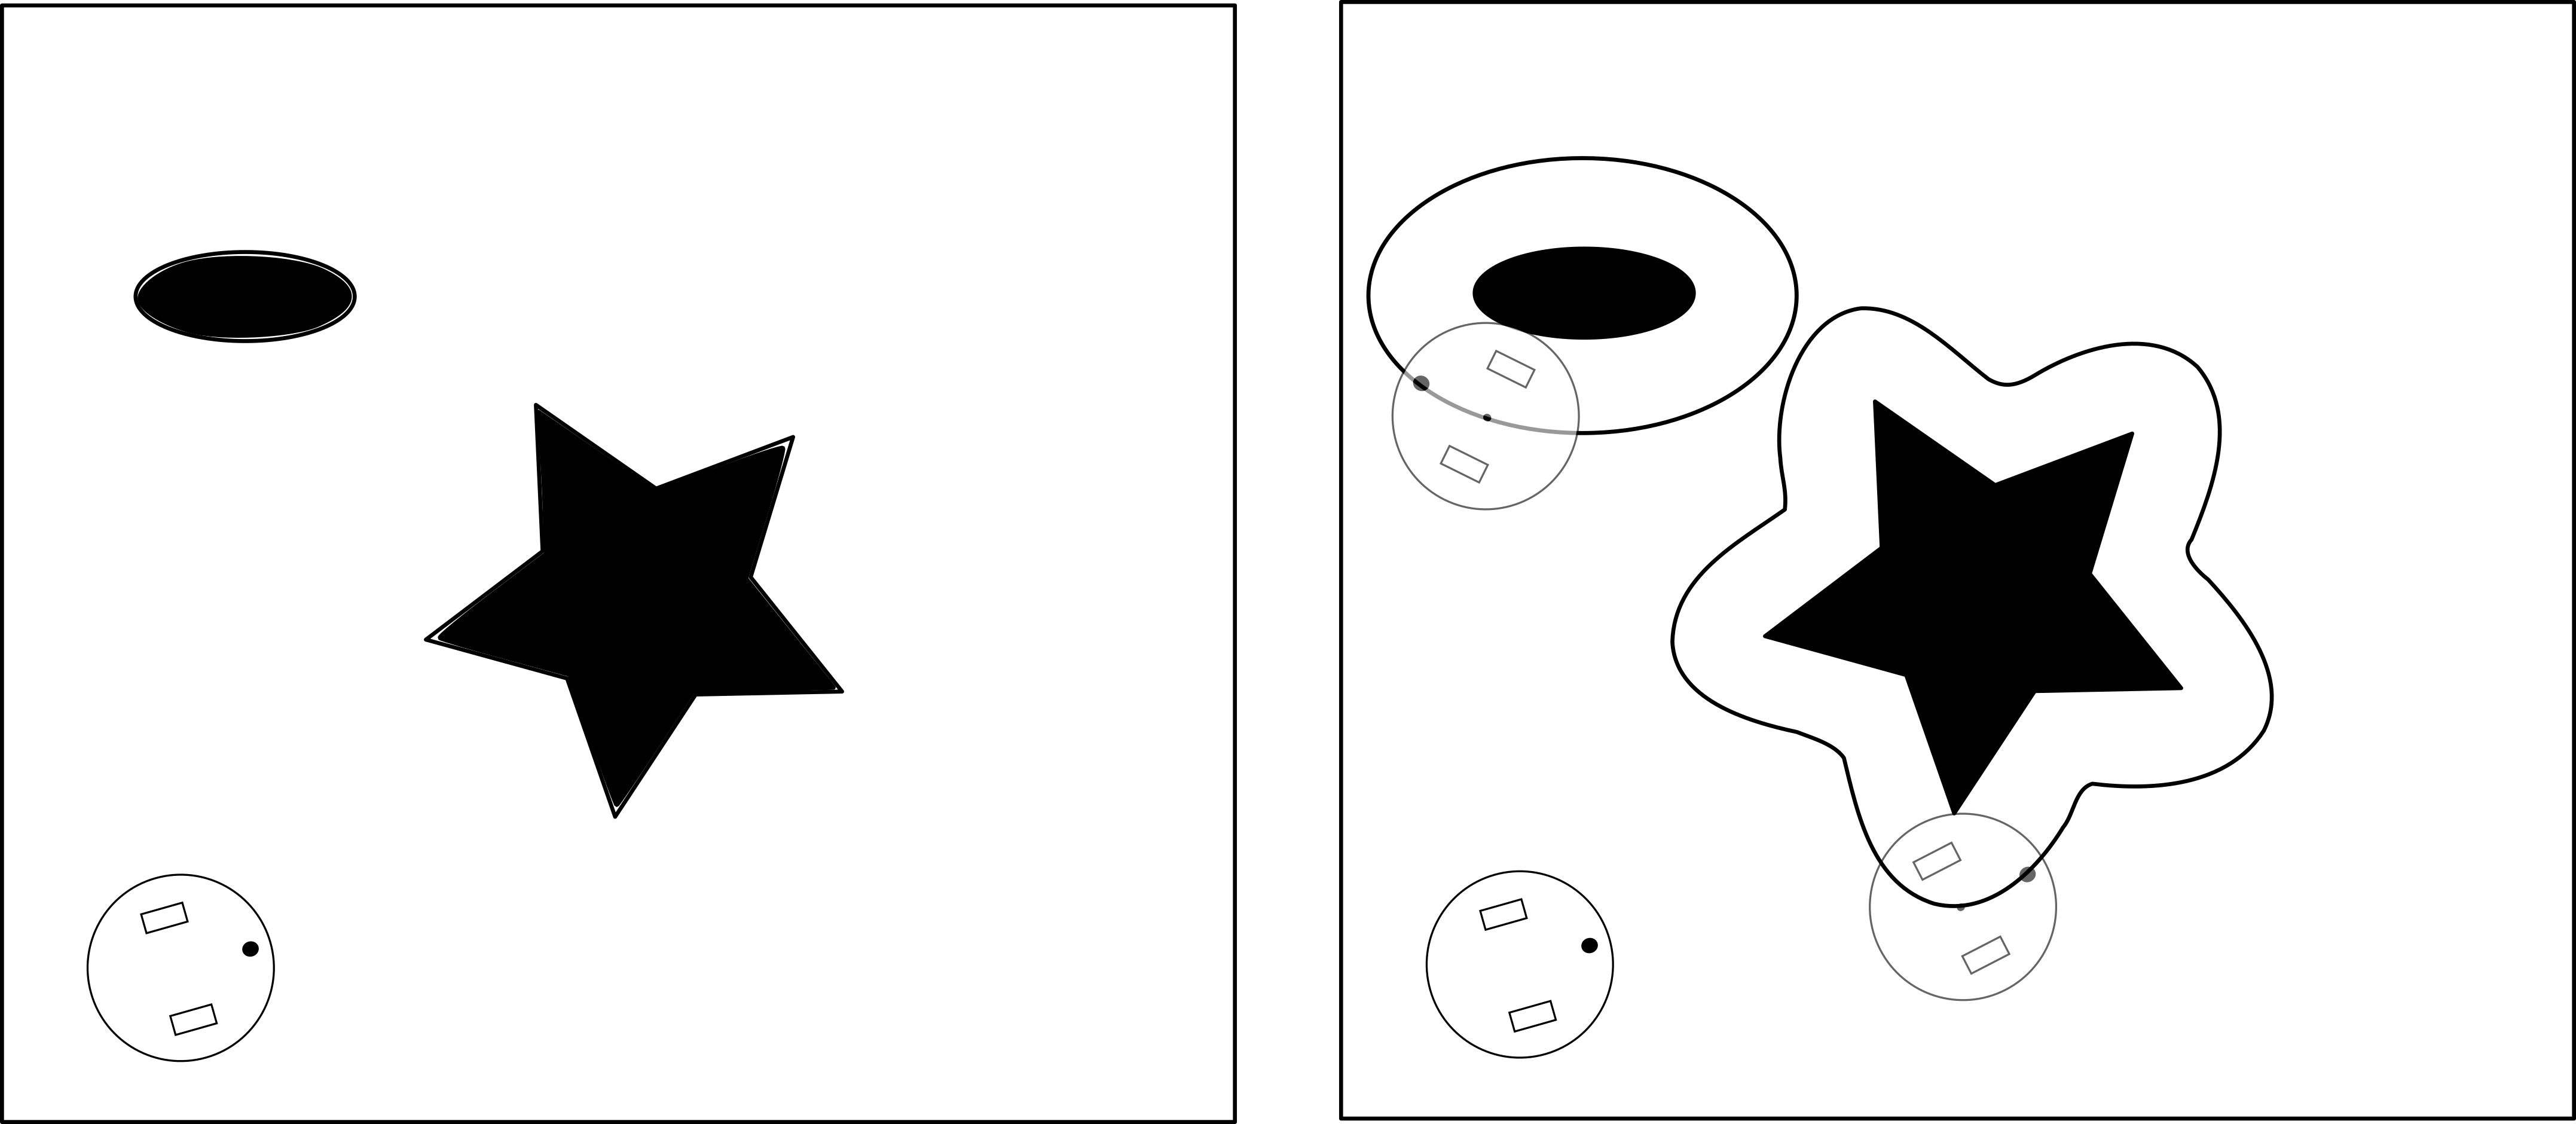
\includegraphics[width=0.9\textwidth]{figs/configurationspace}
\caption{A map with obstacles and its representation in configuration space, which can be obtained by growing each obstacle by the robot's extension. \label{fig:cspace}}
\end{figure}


\subsection{Dijkstra's algorithm}\index{Dijkstra's Shortest Path Algorithm}
One of the earliest and simplest algorithms is Dijkstra's algorithm \cite{dijkstra1959note}. Starting from the initial vertex where the path should start, the algorithm marks all direct neighbors of the initial vertex with the cost to get there. It then proceeds from the vertex with the lowest cost to all of its adjacent vertices and marks them with the cost to get to them via itself if this cost is lower. Once all neighbors of a vertex have been checked, the algorithm proceeds to the vertex with the next lowest cost. Once the algorithm reaches the goal vertex, it terminates and the robot can follow the edges pointing towards the lowest edge cost.

In Figure \ref{fig:pathproblem}, Dijkstra would first mark nodes II, III and IV with cost 3, 5 and 7 respectively. It would then continue to explore all edges of node II, which so far has the lowest cost. This would lead to the discovery that node III can actually be reached in $3+1<5$ steps, and node III would be relabeled with cost 4. In order to completely evaluate node II, Dijkstra needs to evaluate the remaining edge before moving on and label node VI with $3+12=15$.

The node with the lowest cost is now node III (4). We can now relabel node VI with 14, which is smaller than 15, and label node V with $4+5=9$, whereas node IV remains at $4+3=7$. Although we have already found two paths to the goal, one of which better than the other, we cannot stop as there still exist nodes with unexplored edges and overall cost lower than 14. Indeed, continuing to explore from node V leads to a shortest path I-II-III-V-VI of cost 13, with no remaining nodes to explore.

As Dijkstra would not stop until there is no node with lower cost than the current cost to the goal, we can be sure that a shortest path will be found if it exists. We can say that the algorithm is \emph{complete}.\index{Complete (algorithm)}

As Dijkstra will always explore nodes with the least overall cost first, the environment is explored comparably to a wave front originating from the start vertex, eventually arriving at the goal. This is of course highly inefficient in particular if Dijkstra is exploring nodes away from the goal. This can be visualized by adding a couple of nodes to the left of node I in Figure \ref{fig:pathproblem}. Dijkstra will explore all of these nodes until their cost exceeds the lowest found for the goal. This can also be seen when observing Dijkstra's algorithm on a grid, as shown in Figure \ref{fig:dijkstragrid}. 

\begin{figure}[htb]
\centering
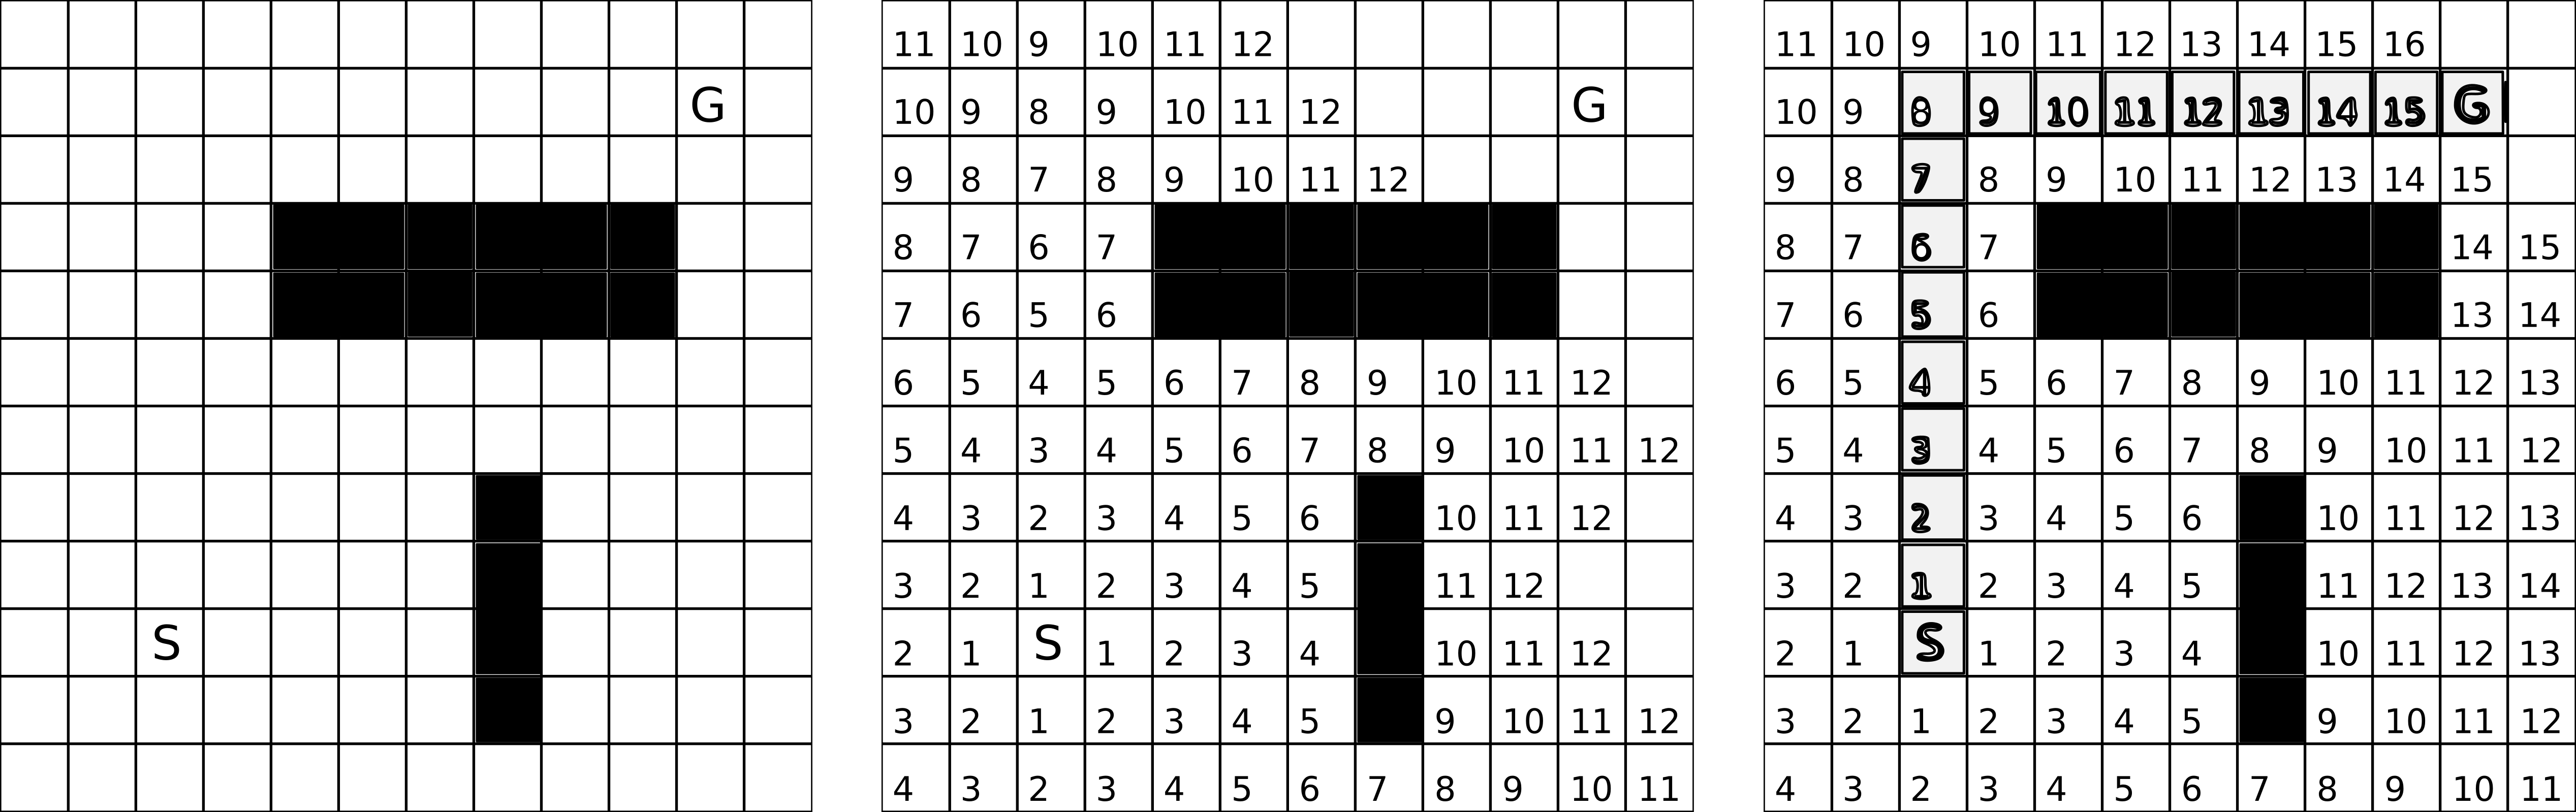
\includegraphics[width=0.9\textwidth]{figs/dijkstragrid}
\caption{Dijkstra's algorithm finding a shortest path from `S' to 'G' assuming the robot can only travel laterally (not diagonally) with cost one per grid cell. Note the few number of cells that remain unexplored once the shortest path (grey) is found, as Dijkstra would always consider a cell with the lowest path cost first.\label{fig:dijkstragrid}}
\end{figure}

\subsection{A*}\label{sec:astar}\index{A* Shortest Path Algorithm}
Instead of exploring in all directions, knowledge of an approximate direction of the goal could help avoiding exploring nodes that are obviously wrong to a human observer. Such special knowledge that such an observer has can be encoded using a \emph{heuristic function}\index{Heuristic function}, a fancier word for a ``rule of thumb''. For example, we could give priority to nodes that have a lower estimated distance to the goal than others. For this, we would mark every node not only with the actual distance that it took us to get there (as in Dijkstra's algorithm), but also with the estimated cost ``as the crow flies'', for example by calculating the Euclidean distance or the \emph{Manhattan distance}\index{Manhattan distance} between the vertex we are looking at and the goal vertex. This algorithm is known as A* \cite{hart1968formal}. Depending on the environment, A* might accomplish search much faster than Dijkstra's algorithm, and performs the same in the worst case. This is illustrated in Figure \ref{fig:astargrid} using the Manhattan distance metric, which does not allow for diagonal movements. 

\begin{figure}[htb]
\centering
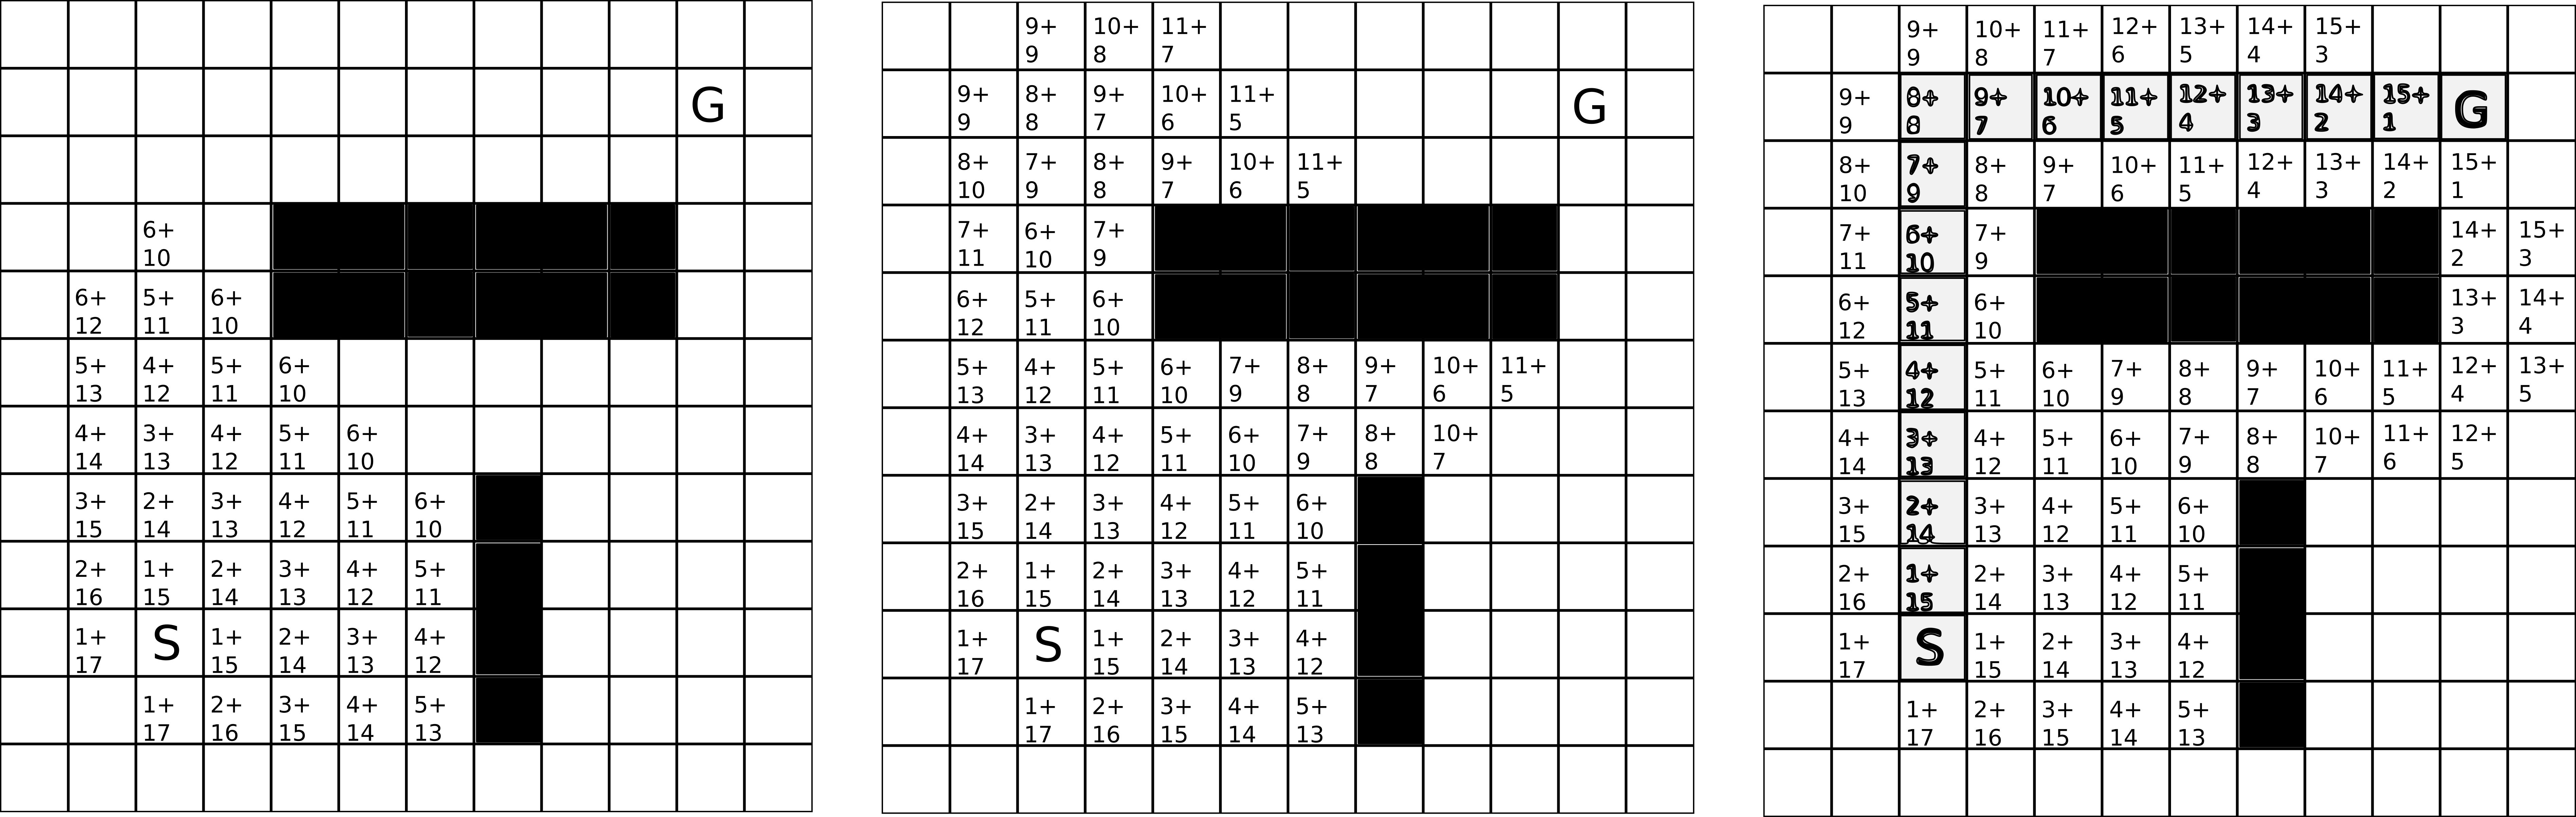
\includegraphics[width=0.9\textwidth]{figs/astargrid}
\caption{Finding a shortest path from `S' to 'G' assuming the robot can only travel laterally (not diagonally) with cost one per grid cell using the A* algorithm. Much like Dijkstra, A* evaluates only the cell with the lowest cost, but takes an estimate of the remaining distance into account.\label{fig:astargrid}}
\end{figure}

An extension of A* that addresses the problem of expensive re-planning when obstacles appear in the path of the robot, is known as D* \cite{stentz1994optimal}. Unlike A*, D* starts from the goal vertex and has the ability to change the costs of parts of the path that include an obstacle. This allows D* to re-plan around an obstacle while maintaining most of the already calculated path.\index{D*}

A* and D* become computationally expensive when either the search space is large, e.g., due to a fine-grain resolution required for the task, or the dimensions of the search problem are high, e.g. when planning for an arm with multiple degrees of freedom. Solutions to these problems are provided by sampling-based path planning algorithms that are described further below.




\section{Sampling-based Path Planning}
The previous sections have introduced a series of complete algorithms for the path planning problem, i.e. they will find a solution eventually if it exists. Complete solutions are often unfeasible, however, when the possible state space is large. This is the case for robots with multiple degrees of freedom such as arms. In practice, most algorithms are only \emph{resolution complete}\index{Resolution complete}, i.e., only complete if the resolution is fine-grained enough, as the state-space needs to be somewhat discretized for them to operate (e.g., into a grid) and some solutions might be missed as a function of the resolution of the discretization.

Instead of evaluating all possible solutions or using a non-complete Jacobian-based inverse kinematic solution, sampling-based planners create possible paths by randomly adding points to a tree until some solution is found or time expires. As the probability to find a path approaches one when time goes to infinity, sampling-based path planners are \emph{probabilistic complete}\index{Probabilistic complete}. Prominent examples of sampling-based planners are \emph{Rapidly-exploring Random Trees} (RRT)\index{Rapidly-exploring Random Tree}\index{RRT}\cite{lavalle1998rapidly} and \emph{Probabilistic Roadmaps}\index{Probabilistic Roadmaps}\index{PRM}(PRM) \cite{kavraki1996probabilistic}. An example execution of RRT for an unknown goal, thereby reducing the path-planning problem to a search problem is shown in Figure \ref{fig:rrt}.

\begin{figure}
\centering
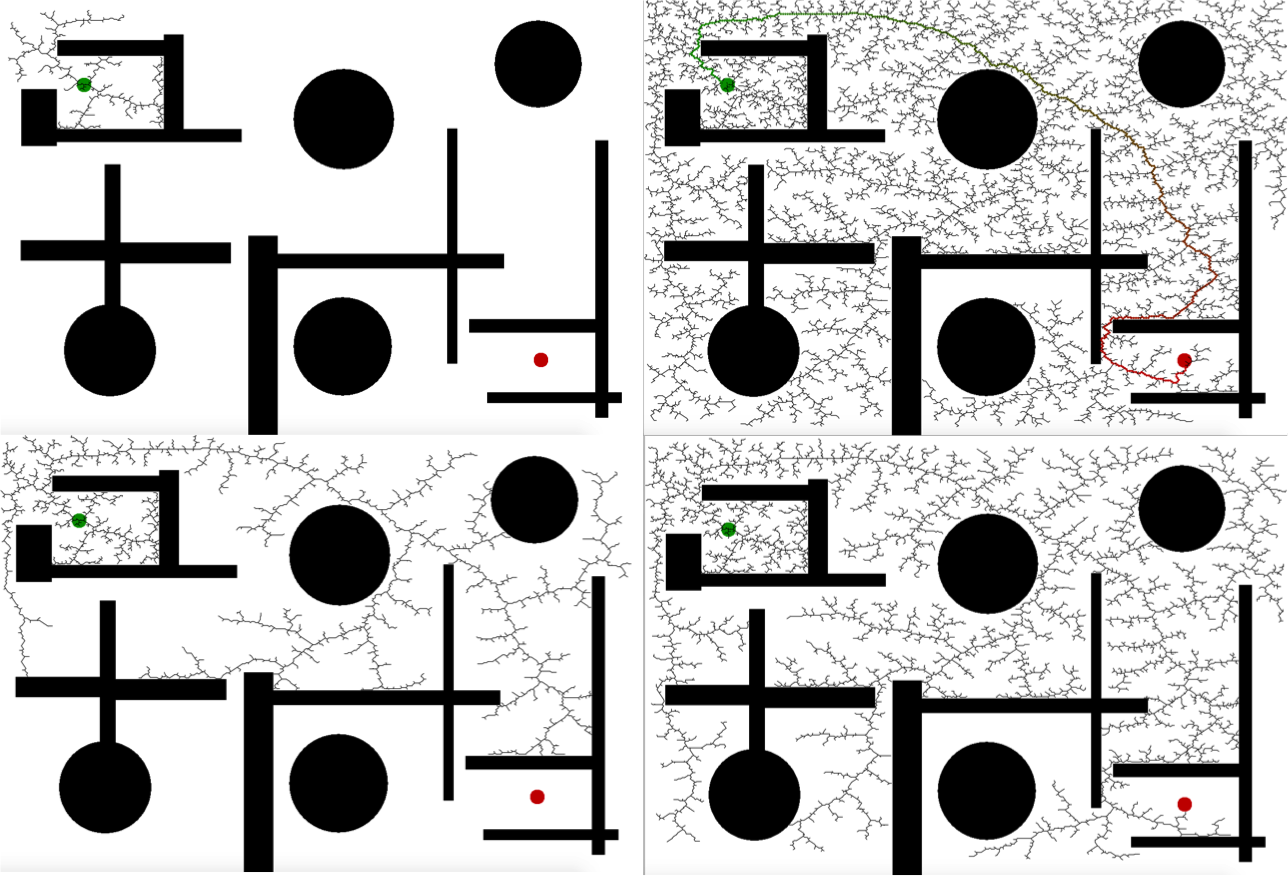
\includegraphics[width=\textwidth]{figs/irrt}
\caption{Counterclockwise: Random exploration of a 2D search space by randomly sampling points and connecting them to the graph until a feasible path between start and goal is found.\label{fig:rrt}}
\end{figure}

This example illustrates well how a sampling-based planner can quickly explore a large portion of space and refines a solution as time goes on. Whereas RRT can be understood as growing a single tree from a robot's starting point until one of its branches hit a goal, probabilistic road-maps create a tree by randomly sampling points in the state-space, testing whether they are collision-free, connecting them with neighboring points using paths that reflect the kinematics of a robot, and then using classical graph shortest path algorithms to find shortest paths on the resulting structure. The advantage of this approach is clearly that such a probabilistic roadmap has to be created only once (assuming the environment is not changing) and can then be used for multiple queries. PRMs are therefore a \emph{multi-query} path-planning algorithm.\index{Multi-query (path-planning)} In contrast, RRT's are known as \emph{single-query}\index{Single-query (path-planning)} path-planning algorithms.

In practice, the boundary between the different historic algorithms has become very diffuse, and single-query and multi-query variants of both RRT and PRM exist. It is important to note that there is no silver bullet algorithm/heuristic and even their parameter-sets are highly problem-specific. We will therefore limit our discussion on useful heuristics that are common to sampling-based planners.

\subsection{Basic Algorithm}
Let $ \mathcal{X}$ be a $ d$-dimensional state-space. This can either be the robot's state given in terms of translation and rotations (6 dimensions), a subset thereof, or the joint space with one dimension per possible joint angle. Let $ \mathcal{G} \subset \mathcal{X}$ be a  d-ball (d-dimensional sphere) in the state-space that is considered to be the goal, and $ t$ the allowed time. A tree planner proceeds as follows:

\begin{verbatim}
Tree=Init(X,start);
WHILE ElapsedTime() < t AND NoGoalFound(G) DO
 newpoint = StateToExpandFrom(Tree);
 newsegment = CreatePathToTree(newpoint);
 IF ChooseToAdd(newsegment) THEN
  Tree=Insert(Tree,newsegment);
 ENDIF
ENDWHILE
return Tree
\end{verbatim}

This process can be repeated on the resulting tree as long as time allows. This is known as an \index{AnyTime algorithm} \emph{AnyTime} algorithm. Given a suitable distance metric, the cost-to-goal can be stored at each node of the tree (much easier if growing the tree from the goal to start), which allows retrieving the shortest path easily. There are four key points in this algorithm:

\begin{enumerate}
\item Finding the next point to add to the tree (or discard) (StateToExpandFrom).
\item Finding out where and how to connect this point to the tree taking into account the robot kinematics (CreatePathToTree).
\item Testing whether this path is suitable, i.e., collision-free.
\item Finding the next point to add.
\end{enumerate}

A prominent method is to pick a random point in the state-space and connect it to the closest existing point in the tree or to the goal. This requires searching all nodes in the tree and calculating their distance to the candidate point. Other approaches put preferences on nodes with fewer out-degrees (those which do not yet have very many connections) and chose a new point within its vicinity. Both approaches make it likely to quickly explore the entire state-space.

If there are constraints imposed on the robot's path, for example the robot needs to hold a cup and therefore is not supposed to rotate its wrist, this dimension can simply be taken out of the state-space.

Once a possible path is found, this space can be reduced to the ellipsoid that bounds the maximal path-length. This ellipsoid can be constructed by mounting a wire of the maximum path length between start and goal and pushing it outward with a pen. All the area that can be reached with the pen constrained by the wire can contain a point that can possibly lead to a shorter path. This approach is particularly effective when running multiple copies of the same planner in parallel and exchanging the shortest paths once they are found \cite{otte2012}.

\subsection{Connecting Points to the Tree}
A new point is classically connected to the closest point already in the tree or to the goal. This can be done by calculating the distance to all points already in the tree. This does not necessarily generate the shortest path, however. A recent improvement has been made by RRT*, which connects the point to the tree in a way that minimizes the overall path length. This can be done by considering all points in the tree within a d-ball (on a 2D map, $d=2$, i.e. a circle) from of fixed radius from the point to add and finding the point that minimizes the overall path length to the start.

Adding a point to the tree is also a good time to take into account the specific kinematics of a robot, for example a car. Here, a local planner can be used to generate a suitable trajectory that takes into account the orientation of the vehicle at each point in the tree.

\subsection{Collision Checking}
Efficient algorithms for testing collisions deserve a dedicated lecture. While the problem is intuitive in configuration-space planning in 2D (the robot reduces to a point) and can be solved using a simple point-in-polygon test, the problem is more involved for manipulators that are subject to self-collision.

As collision checking takes up to 90\% of the execution time in the path planning problem, a successful method to increase computational speed is ``lazy collision evaluation''\index{Lazy collision avoidance}. Instead of checking every point for a possible collision, the algorithm first finds a suitable path. Only then, it checks every segment of this path for collisions. In case some segments are in collision, they are deleted and the algorithm goes on, but keeps the segments of the successful path that were collision-free.

\section{Path Smoothing}
As paths are randomly sampled, they will be most likely shakey and not optimal. For exampe, a grid-map will generate a series of sharp turns and a sampling-based approach will return zig-zag random paths. Results can be drastically improved by running an additional algorithm that smoothes the path. One way of doing this is to connect points of the path using splines, curves or even trajectory snippets that are known to be feasible for a specific platform. Alternatively, one can also use a model of the actual platform and use a feedback controller such as described in Section \ref{sec:fbmobile} for mobile robots and Section \ref{sec:invjac} for arms, sample a series of points in front of the robot, and generate a trajectory that the robot can actually drive. When combined with dynamics, this approach is known as \emph{model-predictive control}\index{Model-predictive control}. Care needs to be taken, however, that the resulting paths are indeed collision free. 

\section{Planning at different length-scales}
In practice, no one map representation and planning algorithm might be sufficient. To plan a route for a car, for example, might involve a coarse search over the street network such as performed by your car's navigation system, but not involve planning which lane to actually choose. Planning lanes and how to navigate round-abouts and intersections will then involve another layer of discrete planning. How to actually move the robot within a lane and avoid local obstacles, might then be best done with a sampling-based planning algorithm. Finally, trajectories need to be turned into wheel speeds and turn angles, possibly using some form of feedback control. This hierarchy is depicted in Figure \ref{fig:planninglayers}. Here, downward-pointing arrays indicate input that one planning layer provides to the one below. Upward-pointing arrows instead indicate exceptions that cannot be handled by the lower levels. For example, a feedback controller cannot handle obstacles well, requiring the sampling-based planning layer to come up with a new trajectory. Should the entire road be blocked, this planner would need to hand-off control the lane-based planner. A similar case can be made for manipulating robots, which also need to combine multiple different representations and controllers to plan and execute trajectories efficiently. 

\begin{figure}
\centering
\includegraphics[width=0.9\textwidth]{figs/planninglayers}
\caption{Path-planning across different length scales, requiring a variety of map representations and planning paradigms. Arrows indicate information passed between layers.\label{fig:planninglayers}}
\end{figure}

Note that this representation does not include a reasoning level that encodes traffic rules and common sense. While some of these might be encoded using cost-functions, such as maximizing distance from obstacles or insuring smooth riding, other more complex behaviors such as adapting driving in the presence of cyclists or properties of the ground need to be implemented in an additional vertical layer that has access to all planning layers. 

\section{Other path-planning applications}
Once the environment has been discretized into a graph, we can employ other algorithms from graph theory to plan desirable robot trajectories. For example, floor coverage can be achieved by performing a depth-first search (DFS) or a breadth-first-search (BFS) on a graph where each vertex has the size of the coverage tool of the robot. ``Coverage'' is not only interesting for cleaning a floor: the same algorithms can be used to perform an exhaustive search of a configuration space, such as in the example shown in Figure \ref{fig:inversekinematics}, where we plotted the error of a manipulator arm in reaching a desired position over its configuration space. Finding a minimum in this plot using an exhaustive search solves the inverse kinematics problem. Similarly, the same algorithm can be used to systematically follow all links on a website till a desired depth (or actually retrieving the entire world-wide web).

Doing a DFS or a BFS might generate efficient coverage paths, but they are far from optimal as many vertices might be visited twice. A path that connects all vertices in a graph but passes every vertex only once is known as a \emph{Hamiltonian Path}.\index{Hamiltonian Path} A Hamiltonian path that returns to its starting vertex is known as a Hamiltonian Cycle. This problem is also known as the Traveling Salesman Problem (TSP), in which a route needs to be calculated that visits every city on his tour only once and is known to be NP Complete.\index{Traveling Salesman Problem}



\section{Summary and Outlook}
Path planning is an ongoing research problem. Finding collision free paths for mechanisms with high degrees of freedom such as multiple arms operating in a common space, multi-robot systems, or systems involving dynamics (and therefore adding the derivatives of the state variables to the planning problem) might take unacceptably long to solve.

Although sampling-based path planners can drastically speed up the time to find some solution, there are not optimal and struggle with specific situations such as narrow passages. There is no ``silver bullet'' algorithm for solving all path planning problems and heuristics that lead to massive speed-up in one scenario might be detrimental in others. Also, algorithmic parameters are mostly ad-hoc and correctly tuning them to a specific environment might drastically increase performance.
 

\section*{Take-home lessons}
\begin{itemize}
\item The first step in path planning is choosing a map representation that is appropriate to the application.
\item The second step is to reduce the robot to a point-mass, which allows planning in the configuration space.
\item This allows the application of generic shortest path finding algorithms, which have applications in a large variety of domains, not limited to robotics.
\item A sampling-based planning algorithm finds paths by sampling random points in the environment. Heuristics are used to maximize the exploration of space and bias the direction of search. This makes these algorithms fast, but neither optimal nor complete.
\item As the resulting paths are random, multiple trials might lead to totally different results.
\item There is no one-size-fits-all algorithm for a path-planning algorithm and care must be taken to select the right paradigm (single-query vs. multi-query), heuristics, and parameters.
\end{itemize}

\section*{Exercises}\small
\begin{enumerate}
\item How does the computational complexity of Dijkstra's algorithm change when moving from 2D to 3D search spaces?
\item A* uses a ``heuristic'' to bias the search in the expected direction of the goal. Why can it only use a heuristic, not the actual length?
\item Assuming points are sampled uniformly at random in a randomized planning algorithm. Calculate the limiting behaviour of the following ratio   (number of points in tree)/(number of points sampled) as the number of points sampled goes to infinity. Assume the total area $A_{total}$ and the area of free space $A_{free}$ within are known. 

\item Assuming a kd-tree is used as a nearest-neighbour data structure, and points are sample uniformly at random, calculate the  run-time of inserting a point into a tree of size $N$. Use ``big-Oh'' notation, e.g. $\mathcal{O}(N)$.

\item What other practical runtime concerns must one consider besides computational complexity alone when doing sampling based motion planning? Can you suggest ways to deal with these other concerns?
\end{enumerate}

\normalsize